\documentclass[article,shortnames]{jss}

%% -- LaTeX packages and custom commands ---------------------------------------

%% recommended packages
\usepackage{orcidlink,thumbpdf,lmodern}

%% another package (only for this demo article)
\usepackage{framed}

%% new custom commands
\newcommand{\class}[1]{`\code{#1}'}
\newcommand{\fct}[1]{\code{#1()}}

%% For Sweave-based articles about R packages:
%% need no \usepackage{Sweave}



%% -- Article metainformation (author, title, ...) -----------------------------

%% - \author{} with primary affiliation (and optionally ORCID link)
%% - \Plainauthor{} without affiliations
%% - Separate authors by \And or \AND (in \author) or by comma (in \Plainauthor).
%% - \AND starts a new line, \And does not.
\author{Alexander Pate~\orcidlink{0000-0002-0849-3458}\\University of Manchester
  \And Matthew Sperrin\\University of Manchester
  \AND Richard D. Riley\\University of Birmingham
  \And Ben Van Calster\\Leiden University\\Medical Centre
  \And Glen P. Martin\\University of Manchester}
\Plainauthor{Alexander Pate, Matthew Sperrin, Ben Van Calster, Richard D. Riley, Glen P. Martin}

%% - \title{} in title case
%% - \Plaintitle{} without LaTeX markup (if any)
%% - \Shorttitle{} with LaTeX markup (if any), used as running title
\title{calibmsm: An \proglang{R} package for calibration plots of the transition probabilities in a multistate model}
\Plaintitle{calibmsm: An R package for calibration plots of the transition probabilities in a multistate model}
\Shorttitle{calibmsm: An \proglang{R} package for calibration plots of a multistate model}

%% - \Abstract{} almost as usual
\Abstract{
  Multistate models, which allow users to answer a wide range of clinical questions, are becoming a more commonly used tool for clinical prediction. It is paramount to evaluate the calibration (as well as other metrics) of a risk prediction model before implementation of the model in practice. Currently no software exists to aid in assessing the calibration of a multistate model. \pkg{calibmsm} has been developed to simplify this process for practicing model developers. Calibration of the transition probabilities between given follow up times is made possible through three approaches. The first two utilise calibration techniques for binary and multinomial logistic regression models in combination with inverse probability of censoring weights, whereas the third utilises psuedo-values. All methods are implemented in conjunction with landmarking.

  This article details the methodology and provides a comprehensive example on how to assess the calibration of a model developed to predict recovery, adverse events, relapse and survival in patients with blood cancer after a transplantation. This is an illustrative example to showcase how to use the package and motivate a discussion around which of the calibration methods is most appropriate.
}

%% - \Keywords{} with LaTeX markup, at least one required
%% - \Plainkeywords{} without LaTeX markup (if necessary)
%% - Should be comma-separated and in sentence case.
\Keywords{clinical prediction, calibration, validation, multistate, multi-state, \proglang{R}}
\Plainkeywords{JSS, style guide, comma-separated, not capitalized, R}

%% - \Address{} of at least one author
%% - May contain multiple affiliations for each author
%%   (in extra lines, separated by \emph{and}\\).
%% - May contain multiple authors for the same affiliation
%%   (in the same first line, separated by comma).
\Address{
  Alexander Pate\\
  Division of Imaging, Informatics and Data Science\\
  Faculty of Biology, Medicine and Health\\
  University of Manchester
  M139PR, UK\\
  E-mail: \email{alexander.pate@manchester.ac.uk}\\
}

\begin{document}


%% -- Introduction -------------------------------------------------------------

%% - In principle "as usual".
%% - But should typically have some discussion of both _software_ and _methods_.
%% - Use \proglang{}, \pkg{}, and \code{} markup throughout the manuscript.
%% - If such markup is in (sub)section titles, a plain text version has to be
%%   added as well.
%% - All software mentioned should be properly \cite-d.
%% - All abbreviations should be introduced.
%% - Unless the expansions of abbreviations are proper names (like "Journal
%%   of Statistical Software" above) they should be in sentence case (like
%%   "generalized linear models" below).

\section[Introduction]{Introduction} \label{sec:intro}

% \begin{leftbar}
% The introduction is in principle ``as usual''. However, it should usually embed
% both the implemented \emph{methods} and the \emph{software} into the respective
% relevant literature. For the latter both competing and complementary software
% should be discussed (within the same software environment and beyond), bringing
% out relative (dis)advantages. All software mentioned should be properly
% \verb|\cite{}|d. (See also Appendix~\ref{app:bibtex} for more details on
% \textsc{Bib}{\TeX}.)
%
% For writing about software JSS requires authors to use the markup
% \verb|\proglang{}| (programming languages and large programmable systems),
% \verb|\pkg{}| (software packages), \verb|\code{}| (functions, commands,
% arguments, etc.). If there is such markup in (sub)section titles (as above), a
% plain text version has to be provided in the {\LaTeX} command as well. Below we
% also illustrate how abbrevations should be introduced and citation commands can
% be employed. See the {\LaTeX} code for more details.
% \end{leftbar}

Risk prediction models enable the prediction of clinical events in either diagnostic or prognostic settings \citep{VanSmeden2021} and are used widely to inform clinical practice. A multistate model \citep{Putter2007} may be used when there are multiple outcomes of interest, or when a single outcome of interest may be reached via intermediates states. Using a multistate model for prediction is important when the development of an intermediate condition occurring post index date may have an impact on the risk of future outcomes of interest. Multistate models are increasingly being developed given the many medical scenarios where modelling patient movement between clinical 'states' is of intrest \citep{Putter2006, Le-Rademacher2018, Lintu2022, Masia2017}. All risk prediction models developed for use in clinical practice should be validated in a relevant cohort prior to implementation \citep{Steyerberg2016, Sperrin2022}. A key part of the validation process is assessment of the calibration of the model \citep{VanCalster2019}. Ideally calibration curves should be produced which allow evaluation of the calibration over the entire distribution of predicted risk, corresponding to moderate assessment of calibration \citep{VanCalster2016}.

The \proglang{R} package \pkg{mstate} \citep{DeWreede2011} provides a comprehensive set of tools to develop a multistate model for a continuously observed multistate survival process. However, currently no software exists to aid researchers in assessing the calibration of a multistate model that has been developed for the purposes of individual risk prediction. \pkg{calibmsm} has been developed to enable researchers to estimate calibration curves and scatter plots using three approaches outlined by Pate et al \textbf{XXXX REF project 6 (may have to put on Arxiv)}, which focused on assessing the calibration of the transition probabilities out of the starting state. The work in this paper extends the framework to assess the calibration of transition probabilities out of any state $j$ at any time $s$ using landmarking \citep{Houwelingen2007, Dafni2011}, provides more details on estimation of the inverse-probability of censoring weights (where relevant), and demonstrates the process for estimating confidence intervals. \pkg{calibmsm} is available from the Comprehensive R Archive Network at \textbf{REF XXXX}.

\cite{DeWreede2011} used data from the European Society for Blood and Marrow Transplantation \citep{EBMT2023} to showcase how to develop a multistate model for clinical prediction of outcomes after bone morrow transplantation in leukemia patients (Figure \ref{fig:msm}). In this study, we show how to assess the calibration of a model developed on the same EBMT data as a way of illustrating the syntax and workflows of \pkg{calibmsm}. This clinical example also highlights some important differences between the methods in how they deal with informative censoring and computational feasibility, which may impact future uptake of the methods. Details on the methodology are given in section 2. The clinical setting for our example and steps for data preparation and are described in section 3. In section 4 we show how to estimate calibration curves and scatter plots using \pkg{calibmsm}. Section 5 contains a discussion and summary.

\begin{figure}
  \centering
  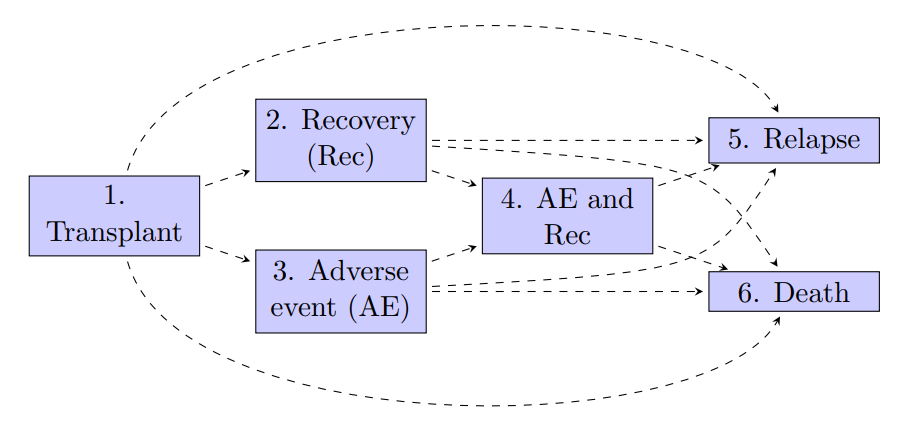
\includegraphics{Figure1.png}
  \caption{\label{fig:msm} A six-state model for leukemia patients after bone marrow transplantation. Figure taken from \citep{DeWreede2011}.}
\end{figure}

%% Section 2: Methodology
\section{Methodology} \label{sec:methodology}

%Sub-section for setup
\subsection{Setup} \label{sec:setup}

Let $X(t) \in \{1, ..., K\}$ be a multistate survival process with $K$ states. We assume a multistate model has already been developed and we want to assess the calibration of the predicted transition probabilities, $\hat{p}_{j,k}(s, t)$, in a cohort of interest. The transition probabilities are the probability of being in state $k$ at time $t$, if in state $j$ at time $s$, where $s$ < $t$. The aim is to estimate observed event probabilities: $$o_{j,k}(s,t) = P[X(t)=k|X(s) = j, \hat{p}_{j,k}(s,t)].$$

In the absence of censoring, this can be done using cross sectional calibration techniques in a landmark \citep{Houwelingen2007, Dafni2011} cohort of individuals who are in state $j$ at time $s$ (i.e. methods to assess the calibration of models predicting binary or polytomous outcomes). In the presence of censoring, calibration must be assessed in this landmark cohort of individuals either using these cross sectional techniques in combination with inverse probability of censoring weights, or through pseudo-values. These approaches are detailed in sections \ref{sec:blripcw} - \ref{sec:sec:ci}.

%Sub-section for BLR-IPCW calibration plots
\subsection{BLR-IPCW calibration curves} \label{sec:blripcw}

The first approach produces calibration curves using a framework for binary logistic regression models with inverse probability of censoring weights (BLR-IPCW). Let $I_{k}(t)$ be an indicator for whether an individual is in state $k$ at time $t$. $I_{k}(t)$ is then modeled using a flexible approach with $\hat{p}_{j, k}(s, t)$ as the sole predictor. This model is fit in the landmark cohort (in state $j$ at time $s$) of individuals uncensored at time $t$, weighted using inverse probability of censoring weights (section \ref{sec:weights}). We suggest using a loess smoother:

\begin{equation}\label{eq:loess}
  I_{k}(t) = \mathrm{loess}(\hat{p}_{j, k}(s, t)),
\end{equation}

or a logistic regression model with restricted cubic splines:

\begin{equation}\label{eq:rcs}
  \mathrm{logit}(I_{k}(t)) = \mathrm{rcs}(\mathrm{logit}(\hat{p}_{j, k}(s, t))).
\end{equation}

Any flexible model for binary outcomes could be used, but these are the most common and are implemented in this package. Observed event probabilities $\hat{o}_{j,k}(s,t)$ are then estimated as fitted values from these models. The calibration curve is plotted using the set of points $\{\hat{p}_{j, k}(s, t), \hat{o}_{j,k}(s,t)\}$. \textbf{This method assumes that in the reweighted population, each outcome $I_{k}(t)$ is independent from the censoring mechanism}.

%Sub-section for MLR-IPCW calibration plots
\subsection{MLR-IPCW calibration plots} \label{sec:mlripcw}

The second approach produces calibration scatter plots using a framework for multinomial logistic regression models with inverse probability of censoring weights (MLR-IPCW). Let $I_{X}(t)$ be an polytomous indicator variable taking values $I_{X}(t) \in \{1, ..., K\}$ such that $I_{X}(t) = k$ if an individual is in state $k$ at time $t$. The nominal recalibration framework of \cite{VanHoorde2014, VanHoorde2015} is then applied in the landmark cohort of individuals uncensored at time $t$, weighted using inverse probability of censoring weights (section \ref{sec:weights}).  First calculate the log-ratios of the predicted transition probabilities:

$$\hat{LP}_{k} = ln\left(\frac{\hat{p}_{j, k}(s, t)}{\hat{p}_{j, k_{ref}}(s, t)}\right),$$

Then fit the following multinomial logistic regression model:

\begin{equation}\label{eq:mlr}
  ln\left(\frac{P[I_{X}(t) = k]}{P[I_{X}(t) = k_{ref}]}\right) = \alpha_{k} + \sum_{h=2}^{K} \beta_{k,h}*s_{k}(\hat{LP}_{h}),
\end{equation}

where $k_{ref}$ is an arbitrary reference category which can be reached from state $j$, $k \neq k_{ref}$ takes values in the set of states that can be reached from state $j$, and where $s$ is a vector spline smoother \citep{Yee2015}. Observed event probabilities $\hat{o}_{j,k}(s,t)$ are then estimated as fitted values from this model. This results in a calibration scatter plot rather than a curve due to all states being modeled simultaneously, as opposed to BLR-IPCW, which is a "one vs all" approach. The scatter occurs because the observed event probabilities for state $k$ vary depending on the predicted transition probabilities of the other states. This is a stronger \citep{VanCalster2016} form of calibration than that evaluated by BLR-IPCW, and will also result in observed event probabilities which sum to 1.\textbf{This method assumes that in the reweighted population, the outcome $I_{X}(t)$ is independent from the censoring mechanism}.

%Sub-section for IPCW weights
\subsection{Estimation of the inverse probability of censoring weights} \label{sec:weights}

The estimand for the weights is $w_{j}(s,t)$, the inverse of the probability of being uncensored at time $t$ if in state $j$ at time $s$:

$$w_{j}(s,t) = \frac{1}{P[t_{cens} > t|t > s, X(s) = j, \textbf{Z},\textbf{X(t)}]},$$

where $\textbf{X(t)}$ denotes the history of the multistate survival process up to time $t$, including the transition times. First the estimator $\hat{P}[t_{cens} > t|t > s, X(s) = j, \textbf{Z}]$ is calculated by developing an appropriate survival model. The outcome in this model is the time until censoring occurs. Moving into an absorbing state prevents censoring from happening and is treated as a censoring mechanism in this model (i.e. a competing risks approach is not taken when fitting this model). $\textbf{X(t)}$ is explicitly conditioned on when defining $w_{j}(s,t)$ because the weights must reflect that censoring can no longer be observed for an individual if they enter an absorbing state at some time $t_{abs} < t$. Therefore

$$\hat{P}[t_{cens} > t|t > s, X(s) = j, \textbf{Z},\textbf{X(t)}] = \hat{P}[t_{cens} > min\{t,t_{abs}\}|t > s, X(s) = j, \textbf{Z}]$$

In \code{calibmsm}, $\hat{P}[t_{cens} > t|t > s, X(s) = j, \textbf{Z}]$ is estimated using a cox proportional hazards model where all predictors $\textbf{Z}$ are assumed to have a linear effect on the log-hazard. However users can also input their own vector of weights. Given the BLR-IPCW and MLR-IPCW approaches are both reliant on correct estimation of the weights, we encourage users to take the time to carefully estimate weights themselves using non-linear models of $\textbf{Z}$ and interaction terms when appropriate.

Stabilised weights can be estimated by multiplying by the weights $w_{j}(s, t)$ by the mean probability of being uncensored:

$$w_{j}^{stab}(s, t) = \frac{P[t_{cens} > t|t > s, X(s) = j]}{P[t_{cens} > t|t > s, X(s) = j, \textbf{Z},\textbf{X(t)}]}.$$

The numerator can be estimated using an intercept only model, and note there is no dependence on $\textbf{X(t)}$.

Another option is to estimate $w(s,t)$, which is the inverse of the probability of being uncensored at time $t$ if uncensored at time $s$:

$$w(s,t) = \frac{1}{P[t_{cens} > t|t > s, \textbf{Z},\textbf{X(t)}]}.$$

This can be estimated using the same approach as for $w_{j}(s,t)$, except there is no requirement to be in state $j$ when landmarking at time $s$. If the censoring mechanism is non-informative after conditioning on the predictors $\textbf{Z}$, then $w(s,t) = w_{j}(s,t)$, and any consistent estimator for $w(s,t)$ will be a consistent estimator of $w_{j}(s,t)$. The advantage is that $\hat{w}(s,t)$ is calculated by developing a model in the cohort of individuals uncensored at time $s$, which is a larger cohort than those uncensored and in state $j$ at time $s$. Therefore $\hat{w}(s,t)$ will be a more precise estimator than $\hat{w}_{j}(s,t)$. On the contrary, if the assumption of non-informative censoring after conditioning on $\textbf{Z}$, there is a risk of bias.

%Sub-section for pseudo-value calibration plots
\subsection{Pseudo-value calibration plots} \label{sec:pseudo}

The third approach produces calibration curves using pseudo-values. Pseudo-values can be used to estimate quantities of interest in censored survival data and multistate survival data. For certain estimators $\hat{\theta}$ (where $\theta$ must take the form of an expectation), the pseudo-value for individual $i$ is defined as:

$$\hat{\theta}^{i} = n*\hat{\theta} - \left(n-1\right)*\hat{\theta}^{-i},$$

where $\hat{\theta}^{-i}$ is equal to $\hat{\theta}$ estimated in a cohort without individual $i$. One such estimator for the transition probabilities in a multistate model, $P[X(t)=k|X(s) = j]$, is the Landmark Aalen-Johansen estimator \citep{Putter2018}. Note that this is equivalent to landmarking the cohort and estimating the Aalen-Johansen estimator \citep{Aalen1978}, which is what's done in this package. The resulting pseudo-values are vectors with $K$ elements, one for each possible transition. These pseudo-values can replace the outcome $I_{k}(t)$ in equations (\ref{eq:loess}) and (\ref{eq:rcs}) in order to estimate $o_{j,k}(s,t)$.

However, the pseudo-values are based on the same assumptions as the underlying estimator $\hat{\theta}$. The Landmark Aalen-Johansen estimator requires non-informative censoring. The approach to alleviate this is to estimate the pseudo-values within sub-groups of individuals, now making the assumption that censoring is non-informative within the specified subgroups. This can be done by calculating the pseudo-values within subgroups defined by baseline predictors, or subgroups defined by the predicted transition probabilities of state $k$. Both options are implemented in this package. whether the pseudo-values are calculated within subgroups or not, they are used as the outcome in models (\ref{eq:loess}) and (\ref{eq:rcs}) in the same way. Note that the pseudo-values $\hat{\theta}^{i}$ are continuous, as opposed to binary $I_{k}(t)$, but the link function in model (\ref{eq:rcs}) remains the same to ensure $\hat{o}_{j,k}(s,t)$ are between zero and one.

%Sub-section for estimation of confidence intervals
\subsection{Estimation of confidence intervals} \label{sec:ci}

Confidence intervals for both BLR-IPCW and pseudo-value calibration curves can be estimated using bootstrapping. A process for estimating the confidence intervals around the BLR-IPCW calibration curves is as follows:

\begin{enumerate}
 \item Resample validation dataset with replacement
 \item Landmark the dataset for assessment of calibration
 \item Calculate inverse probability of censoring weights
 \item Fit the preferred calibration model in the landmarked dataset (restricted cubic splines or loess smoother)
 \item Generate observed event probabilities for a fixed vector of predicted transition probabilities (specifically the predicted transition probabilities from the non-bootstrapped landmark validation dataset)
\end{enumerate}

This will produce a number of bootstrapped calibration curves, all plotted over the same vectors of predicted transition probabilities. Taking the $\frac{\alpha}{2}$ and $\left(1-\frac{\alpha}{2}\right)$ percentiles of the observed event probabilities for each predicted transition probability gives the required $1-\alpha$ confidence interval around the estimated calibration curve. To estimate confidence intervals for the pseudo-value calibration curves using bootstrapping, the same procedure is applied except the third step is replaced with 'calculate the pseudo-values within the landmarked bootstrapped dataset'. For the pseudo-value approach, this will be highly computationally demanding as the pseudo-values must be estimated in every bootstrap dataset.

If using the pseudo-value method, confidence intervals can be calculated using parametric estimates of the standard error when making predictions of the observed event probabilities (i.e. when making predictions from model (\ref{eq:loess}) or (\ref{eq:rcs})). To obtain a parametric confidence interval when using the BLR-IPCW approach, a robust sandwich-type estimator should be used to estimate the standard error \citep{Hernan2020}. In \pkg{calibmsm}, this has been implemented for calibration curves estimated using restricted cubic splines. However, a sandwich estimator was shown to be biased when estimating the standard error of a treatment effect when using inverse probability of treatment weighting in survival analysis \citep{Austin2016}. The performance of robust sandwich-type estimators when using inverse probability of censoring weights in a binary logistic regression is still relatively unknown \textbf{I'm struggling to find references on this}. Furthermore, the size of the confidence interval will be underestimated as uncertainty in estimation of the weights is not considered, which is more of an issue at small sample sizes.

Both the parametric and bootstrap methods have been built into \pkg{calibmsm}. However for the reasons outlined above, we recommend using parametric confidence intervals for the pseudo-value calibration curves and bootstrapping for the BLR-IPCW calibration curves.

%% Section 3: Data preperation
\section{Clinical setting and data preperation} \label{sec:dataprep}

We utilise data from the European Society for Blood and Marrow Transplantation \citep{EBMT2023}, containing multistate survival data after a transplant for patients with blood cancer. The start of follow up is the day of the transplant and the initial state is alive and in remission. There are three intermediate events ($2$: recovery, $3$: adverse event, or $4$: recovery + adverse event), and two absorbing states ($5$: relapse and $6$: death). This data is available from the \pkg{mstate} package \citep{DeWreede2011}.

Four datasets are provided to enable assessment of a multistate model fitted to these data. The first is \code{ebmtcal}, which is the same as the \code{ebmt} dataset provided in \pkg{mstate} , with two extra variables derived: time until censoring (\code{dtcens}) and an indicator for whether censoring was observed (\code{dtcens.s = 1}) or an absorbing state was entered (\code{dtcens.s = 0}). This dataset contains baseline information on year of transplant (\code{year}), age at transplant (\code{age}), prophylaxis given (\code{proph}), and whether the donor was gender matched (\code{match}). The second dataset provided is \code{msebmtcal}, which is the \code{ebmt} dataset converted into \code{msdata} format using the process outlined in \cite{DeWreede2011}. It contains all transition times, an event indicator for each transition, as well as a \code{trans} attribute containing the transition matrix.

\begin{Schunk}
\begin{Sinput}
R> library("calibmsm")
R> data("ebmtcal")
R> head(ebmtcal)
\end{Sinput}
\begin{Soutput}
  id  rec rec.s   ae ae.s recae recae.s  rel rel.s  srv srv.s
1  1   22     1  995    0   995       0  995     0  995     0
2  2   29     1   12    1    29       1  422     1  579     1
3  3 1264     0   27    1  1264       0 1264     0 1264     0
4  4   50     1   42    1    50       1   84     1  117     1
5  5   22     1 1133    0  1133       0  114     1 1133     0
6  6   33     1   27    1    33       1 1427     0 1427     0
       year agecl proph              match dtcens dtcens.s
1 1995-1998 20-40    no no gender mismatch    995        1
2 1995-1998 20-40    no no gender mismatch    422        0
3 1995-1998 20-40    no no gender mismatch   1264        1
4 1995-1998 20-40    no    gender mismatch     84        0
5 1995-1998   >40    no    gender mismatch    114        0
6 1995-1998 20-40    no no gender mismatch   1427        1
\end{Soutput}
\begin{Sinput}
R> data("msebmtcal")
R> head(msebmtcal)
\end{Sinput}
\begin{Soutput}
  id from to trans Tstart Tstop time status
1  1    1  2     1      0    22   22      1
2  1    1  3     2      0    22   22      0
3  1    1  5     3      0    22   22      0
4  1    1  6     4      0    22   22      0
5  1    2  4     5     22   995  973      0
6  1    2  5     6     22   995  973      0
\end{Soutput}
\end{Schunk}

In the work of \cite{DeWreede2011}, the focus is on predicting transition probabilities made at times $s = 0$ and $s = 100$ across a range of follow up times $t$, and comparing prognosis for patients in different states $j$. In this study we also focus on assessing the calibration of the transition probabilities made at these times. We assess calibration of the transition probabilities at $t = 5$ years, a common follow up time for cancer prognosis, but calibration of the model may vary for other values of $t$. We estimate transition probabilities for each individual by developing a model as demonstrated in \cite{DeWreede2011}, following the theory of \cite{Putter2007}. The predicted transitions probabilities from each state $j$ at times $s = 0$ and $s = 100$ are contained in stacked datasets \code{tps0} and \code{tps100} respectively. A leave-one-out approach was used when estimating these transition probabilities. This means each individual was removed from the development dataset when fitting the multistate model to estimator their transition probabilities. This approach allows validation to be assessed in the same dataset that the model was developed with minimal levels of in-sample optimism. The code for deriving all these datasets is provided in the source code for \pkg{calibmsm}.

\begin{Schunk}
\begin{Sinput}
R> data("tps0")
R> head(tps0)
\end{Sinput}
\begin{Soutput}
  id   pstate1   pstate2    pstate3   pstate4   pstate5   pstate6
1  1 0.1139726 0.2295006 0.08450376 0.2326861 0.1504855 0.1888514
2  2 0.1140189 0.2316569 0.08442692 0.2328398 0.1481977 0.1888598
3  3 0.1136646 0.2317636 0.08274331 0.2325663 0.1504787 0.1887834
4  4 0.1383878 0.1836189 0.07579429 0.2179331 0.1538475 0.2304185
5  5 0.1233226 0.1609740 0.05508100 0.1828176 0.1425950 0.3352099
6  6 0.1136646 0.2317636 0.08462424 0.2305854 0.1505534 0.1888087
         se1        se2        se3        se4        se5        se6 j
1 0.01291133 0.02369584 0.01257251 0.02323376 0.01648630 0.01601795 1
2 0.01291552 0.02374329 0.01256056 0.02324869 0.01632797 0.01603703 1
3 0.01289444 0.02375770 0.01245752 0.02322375 0.01647890 0.01601525 1
4 0.01857439 0.03004447 0.01462570 0.03018673 0.02124071 0.02416121 1
5 0.01944967 0.03419721 0.01367768 0.03423941 0.02329644 0.03688586 1
6 0.01289444 0.02375770 0.01257276 0.02317348 0.01649531 0.01602438 1
\end{Soutput}
\begin{Sinput}
R> data("tps100")
R> head(tps100)
\end{Sinput}
\begin{Soutput}
  id   pstate1    pstate2 pstate3 pstate4   pstate5   pstate6
1  1 0.7013881 0.05239271       0       0 0.1408120 0.1054072
2  2 0.7012745 0.05261136       0       0 0.1407625 0.1053516
3  3 0.7011368 0.05270176       0       0 0.1407628 0.1053987
4  4 0.6840325 0.04139266       0       0 0.1700565 0.1045183
5  5 0.6804049 0.04308434       0       0 0.1500344 0.1264764
6  6 0.7011368 0.05270176       0       0 0.1407628 0.1053987
         se1        se2 se3 se4        se5        se6 j
1 0.04691168 0.02077138   0   0 0.03457006 0.03081258 1
2 0.04691218 0.02082871   0   0 0.03456448 0.03079617 1
3 0.04693068 0.02086917   0   0 0.03456101 0.03081033 1
4 0.05885230 0.02161973   0   0 0.04710517 0.03673242 1
5 0.06694739 0.02484634   0   0 0.04905043 0.04628088 1
6 0.04693068 0.02086917   0   0 0.03456101 0.03081033 1
\end{Soutput}
\end{Schunk}

%% Section 4: Calibration curves and scatter plots
\section[Assessing calibration using calibration curves and scatter plots]{Assessing calibration using calibration curves and scatter plots} \label{sec:calibplots}

The procedure for producing calibration plots requires the use of two functions. The first function, \code{calib_blr}, \code{calib_pv} or \code{calib_mlr}, calculates the data for the calibration plot using the methods described in section \ref{sec:methodology}. The second function, \code{plot.calib_blr}, \code{plot.calib_pv} or \code{plot.calib_mlr}, produces the plots using \pkg{ggplot2}. Separating these processes allows users the flexibility of producing their own Figures once the calibration data has been estimated.

The functions for estimating the calibration curves have three arguments where the data provided must be in a specific format. The \code{data.mstate} argument requires an object of class \code{msdata}, and is used to implement the landmarking. A dataset of this class must be produced using the package \pkg{mstate} \citep{DeWreede2011}. The \code{data.raw} argument requires a \code{data.frame} (one observation per individual) and is used to fit the calibration models. For methods BLR-IPCW and MLR-IPCW, \code{data.raw} should contain variables \code{dtcens} (censoring time) and \code{dtcens.s} (censoring indicator, \code{dtcens.s = 1} if the individual is censored at time \code{dtcens}, \code{dtcens.s = 0} otherwise), plus any baseline predictors $\textbf{Z}$ used to estimate the weights. For the pseudo-value approach, this dataset should contain any baseline predictors $\textbf{Z}$ which variables will be grouped by before calculating the pseudo-values. Both \code{data.mstate} and \code{data.raw} should contain a patient ID variable \code{id}. The \code{tp.pred} argument must contain a column for each transition $k$, even if the transition from $j$ to $k$ has zero probability. Each row in \code{tp.pred} should correspond to the equivalent row in \code{data.raw}. The datasets described in section \ref{sec:dataprep} meet these criteria.

%% Subsection for j = 1, s = 0
\subsection[Plots out of states j = 1 at time s = 0]{Plots out of state $j = 1$ at time $s = 0$} \label{sec:plotsj1s0}

We start by producing calibration curves for the predicted transition probabilities out of state $j = 1$ at time $s = 0$. Given all individuals start in state $1$, there is no need to consider the transition probabilities out of states $j \neq 1$ at $s = 0$. Calibration is assessed at follow up time ($t = 1826$ days). We first evaluate calibration using the BLR-IPCW approach, implemented through the function \code{calib_blr}.

The predicted transition probabilities from state $j = 1$ at time $s = 0$ (\code{tp.pred}) are extracted from the object \code{tps0}. We choose to estimate the calibration curves using restricted cubic splines, and 3 knots are chosen given the reasonably small size of the dataset. Weights are estimated using the internal estimation procedure and the predictor variables \code{year}, \code{agecl}, \code{proph} and \code{match}. The \code{w.landmark.type} argument assigns whether weights are estimated using all individuals uncensored at time $s$, or only those uncensored and in state $j$ at time $s$, as discussed in section \ref{sec:weights}. The maximum weight (\code{w.max = 10}) and stabilisation of weights (\code{stabilised = FALSE}) are left as default. Weights can also be manually specified using the \code{weights} argument. We request 95\% confidence intervals for the calibration curves calculated through bootstrapping with 200 bootstrap replicates.

\begin{Schunk}
\begin{Sinput}
R> t.eval <- 1826
R> dat.calib.blr <-
+    calib_blr(data.mstate = msebmtcal,
+                   data.raw = ebmtcal,
+                   j=1,
+                   s=0,
+                   t.eval = t.eval,
+                   tp.pred = tps0 |>
+                     dplyr::filter(j == 1) |>
+                     dplyr::select(any_of(paste("pstate", 1:6, sep = ""))),
+                   curve.type = "rcs",
+                   rcs.nk = 3,
+                   w.covs = c("year", "agecl", "proph", "match"),
+                   CI = 95,
+                   CI.R.boot = 200)
\end{Sinput}
\end{Schunk}

The first element of \code{dat.calib.blr} (named \code{plotdata}) contains 6 data frames for the calibration curves of the transition probabilities into each of the six states, $k \in \{1,2,3,4,5,6\}$. Each data frame contains three columns, \code{id}: the identifier of each individual; \code{pred}: the predicted transition probabilities; \code{obs}: the observed event probabilities. These data frames have less rows than \code{ebmtcal} because calibration can only be assessed in individuals uncensored at time \code{t.eval} \textbf{replace t.eval with t}. The second element (named \code{metadata}) is a metadata argument containing a vector of the possible transitions from state $j$ (all states cannot necessarily be reached from state $j$), the size of the confidence interval (currently \code{false}), and the type of calibration curve (\code{rcs} or \code{loess}).

\begin{Schunk}
\begin{Sinput}
R> str(dat.calib.blr[["plotdata"]])
\end{Sinput}
\begin{Soutput}
List of 6
 $ state1:'data.frame':	1778 obs. of  5 variables:
  ..$ id       : int [1:1778] 2 4 5 7 10 13 14 16 18 19 ...
  ..$ pred     : num [1:1778] 0.114 0.1384 0.1233 0.0974 0.1137 ...
  ..$ obs      : num [1:1778] 0.11 0.104 0.105 0.124 0.11 ...
  ..$ obs.lower: num [1:1778] 0.0877 0.0796 0.0836 0.0877 0.0879 ...
  ..$ obs.upper: num [1:1778] 0.128 0.126 0.123 0.16 0.128 ...
 $ state2:'data.frame':	1778 obs. of  5 variables:
  ..$ id       : int [1:1778] 2 4 5 7 10 13 14 16 18 19 ...
  ..$ pred     : num [1:1778] 0.232 0.184 0.161 0.212 0.232 ...
  ..$ obs      : num [1:1778] 0.17 0.186 0.176 0.179 0.17 ...
  ..$ obs.lower: num [1:1778] 0.12 0.157 0.146 0.144 0.12 ...
  ..$ obs.upper: num [1:1778] 0.232 0.22 0.209 0.211 0.232 ...
 $ state3:'data.frame':	1778 obs. of  5 variables:
  ..$ id       : int [1:1778] 2 4 5 7 10 13 14 16 18 19 ...
  ..$ pred     : num [1:1778] 0.0844 0.0758 0.0551 0.0615 0.0844 ...
  ..$ obs      : num [1:1778] 0.1249 0.1167 0.0919 0.1001 0.1248 ...
  ..$ obs.lower: num [1:1778] 0.1008 0.0911 0.0459 0.0584 0.1008 ...
  ..$ obs.upper: num [1:1778] 0.156 0.149 0.145 0.146 0.156 ...
 $ state4:'data.frame':	1778 obs. of  5 variables:
  ..$ id       : int [1:1778] 2 4 5 7 10 13 14 16 18 19 ...
  ..$ pred     : num [1:1778] 0.233 0.218 0.183 0.221 0.233 ...
  ..$ obs      : num [1:1778] 0.243 0.224 0.185 0.228 0.243 ...
  ..$ obs.lower: num [1:1778] 0.204 0.195 0.16 0.196 0.204 ...
  ..$ obs.upper: num [1:1778] 0.281 0.257 0.223 0.261 0.281 ...
 $ state5:'data.frame':	1778 obs. of  5 variables:
  ..$ id       : int [1:1778] 2 4 5 7 10 13 14 16 18 19 ...
  ..$ pred     : num [1:1778] 0.148 0.154 0.143 0.144 0.149 ...
  ..$ obs      : num [1:1778] 0.191 0.165 0.222 0.212 0.188 ...
  ..$ obs.lower: num [1:1778] 0.164 0.149 0.175 0.172 0.163 ...
  ..$ obs.upper: num [1:1778] 0.215 0.185 0.267 0.25 0.211 ...
 $ state6:'data.frame':	1778 obs. of  5 variables:
  ..$ id       : int [1:1778] 2 4 5 7 10 13 14 16 18 19 ...
  ..$ pred     : num [1:1778] 0.189 0.23 0.335 0.264 0.189 ...
  ..$ obs      : num [1:1778] 0.207 0.254 0.316 0.28 0.207 ...
  ..$ obs.lower: num [1:1778] 0.183 0.225 0.275 0.252 0.183 ...
  ..$ obs.upper: num [1:1778] 0.229 0.283 0.361 0.31 0.229 ...
\end{Soutput}
\begin{Sinput}
R> str(dat.calib.blr[["metadata"]])
\end{Sinput}
\begin{Soutput}
List of 8
 $ valid.transitions   : num [1:6] 1 2 3 4 5 6
 $ assessed.transitions: num [1:6] 1 2 3 4 5 6
 $ CI                  : num 95
 $ CI.R.boot           : num 200
 $ curve.type          : chr "rcs"
 $ j                   : num 1
 $ s                   : num 0
 $ t.eval              : num 1826
\end{Soutput}
\end{Schunk}

Calibration curves can then be generated using \code{plot.calib_blr}. This S3 generic was written for objects of class \code{calib_blr} and produces the calibration plots using \pkg{ggplot2}. The calibration curves (Figure \ref{fig:blrj1s0}) indicate the level of calibration is different for the transition probabilities into each of the different states. The calibration into states $4$ and $6$ is good, as both contain the line of prefect calibration across the entire range of predicted risk. State $2$ has good calibration over the majority of the predicted risks but over predicts for individuals with the highest predicted risks. Transition probabilities into states $1$ and $3$ are over and under predicted respectively over most of the range of predicted risks, and large portions of the confidence intervals do not contain the line of perfect calibration. Importantly the calibration of the transition probabilities into state $5$ (Relapse), a key clinical outcome in this clinical setting, is extremely poor.

\begin{figure}[t!]
\centering
\begin{Schunk}
\begin{Sinput}
R> plot(dat.calib.blr, combine = TRUE, nrow = 2, ncol = 3)
\end{Sinput}
\end{Schunk}
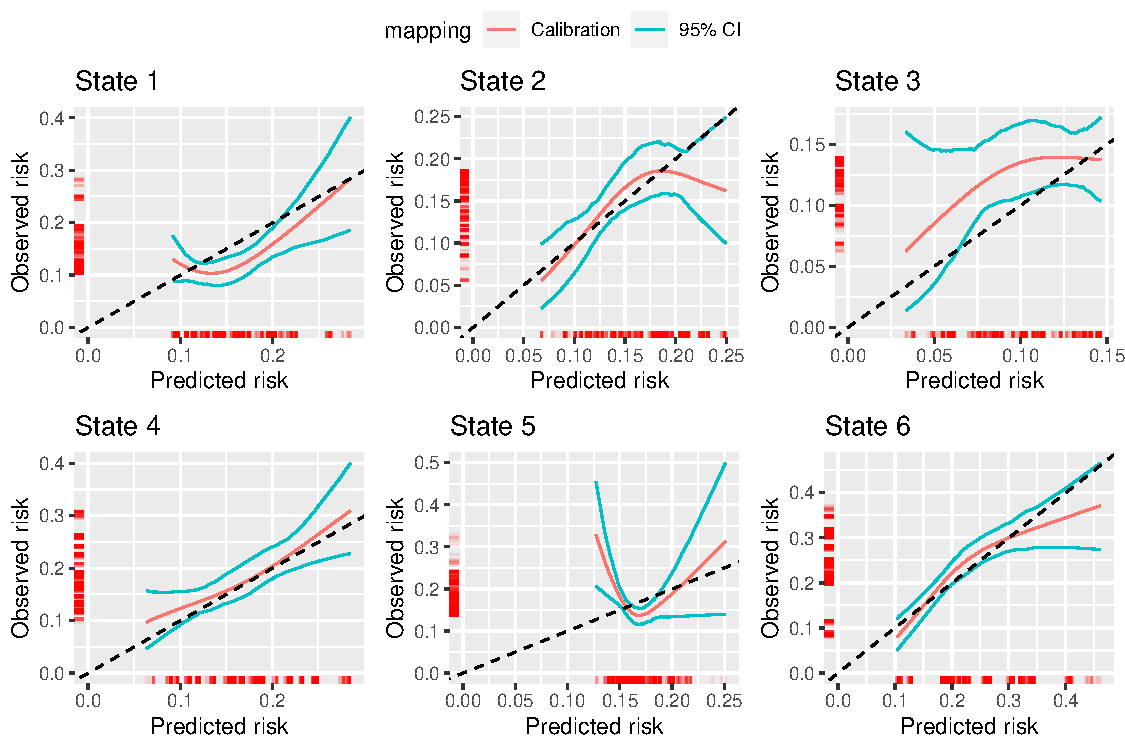
\includegraphics{calibmsm-jss-TEST-006}
\caption{\label{fig:blrj1s0} BLR-IPCW calibration curves out of state j =  1 at time s = 0.}
\end{figure}

Next we use the pseudo-value approach to assess calibration, implemented through the function \code{calib_pv}. Instead of specifying how the weights are estimated, we now specify variables to define groups within which pseudo-values will be calculated (see section \ref{sec:pseudo}). We choose to calculate pseudo-values within individuals with the same year of transplant (\code{group.vars}), and then split individuals into a further three groups defined by their predicted risk (\code{n.pctls}). The number of percentiles should be increased in bigger validation datasets. Year of transplant was identified as a subgrouping variable through exploration of the dataset (supplementary material XXXX). A later transplant resulted in a shorter possible follow up, an earlier administrative censoring time, and it was therefore highly predictive of the probability of being censored. A parametric confidence interval is estimated as recommended in section \ref{sec:ci}.

\begin{Schunk}
\begin{Sinput}
R> dat.calib.pv <-
+    calib_pv(data.mstate = msebmtcal,
+                  data.raw = ebmtcal,
+                  j=1,
+                  s=0,
+                  t.eval = t.eval,
+                  tp.pred = tps0 |>
+                   dplyr::filter(j == 1) |>
+                   dplyr::select(any_of(paste("pstate", 1:6, sep = ""))),
+                  curve.type = "rcs",
+                  rcs.nk = 3,
+                  group.vars = c("year"),
+                  n.pctls = 3,
+                  CI = 95,
+                  CI.type = "parametric")
\end{Sinput}
\end{Schunk}

Calibration curves were then generated using \code{plot.calib_pv}. The pseudo-value calibration curves (Figure \ref{fig:pvj1s0}) are largely similar to the BLR-IPCW calibration curves (Figure \ref{fig:blrj1s0}). The agreement in the calibration curves from two completely distinct methods provides reassurance the assessment of calibration is correct. This is with the exception of state $k = 3$, where the pseudo-value calibration plot indicates the transition probabilities are well calibrated, but the BLR-IPCW calibration plot indicates the transition probabilities under predict. If developing this model in a clinical setting, further exploration of this difference would be required. In particular, how the variable year of transplant acts on the censoring mechanism, and for which method the assumptions about independence of the censoring mechanism (section \ref{sec:methodology}) are most likely to hold.

\textbf{I could delve into this a bit more deeply. I think the pseudo-value method is probably more appropriate, as I reckon the model for estimating the weights in} \code{calib_blr} \textbf{is probably misspecified as the proportional hazard assumption unlikely to hold within levels of year of transplant. This then leads to a conversation around why the BLR-IPCW plot and pseudo-value plot are the same for all other states. I think possibly because state 3 has some odd properties, in that patients may not move into state 3 after 100 days. I think this discussion is valuable, as it highlights the need to correct specify weights/review the assumptions of each method, but also wary of over complicating this paper.}

\begin{figure}
\centering
\begin{Schunk}
\begin{Sinput}
R> plot(dat.calib.pv, combine = TRUE, nrow = 2, ncol = 3)
\end{Sinput}
\end{Schunk}
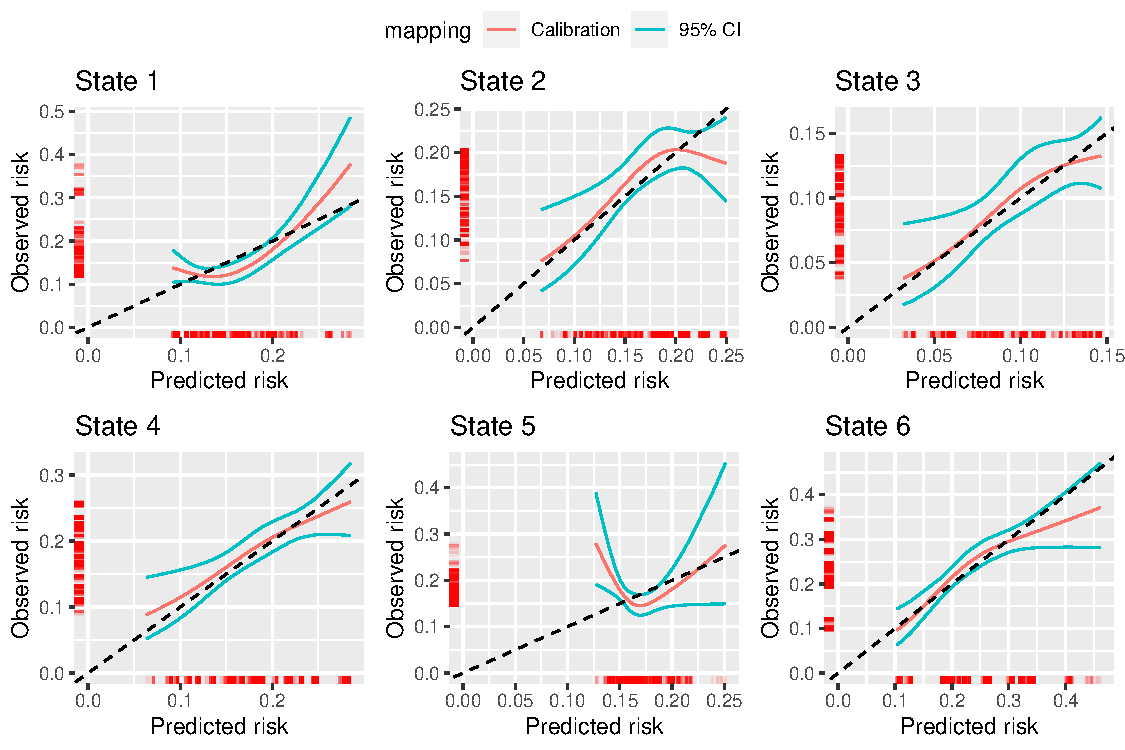
\includegraphics{calibmsm-jss-TEST-008}
\caption{\label{fig:pvj1s0} Pseudo-value calibration curves out of state j =  1 at time s = 0.}
\end{figure}

Next we use the MLR-IPCW to evaluate calibration which produces a calibration scatter plot. This is done using the \code{calib_mlr} function, which has the same inputs as \code{calib_blr}.

\begin{Schunk}
\begin{Sinput}
R> dat.calib.mlr <-
+    calib_mlr(data.mstate = msebmtcal,
+                   data.raw = ebmtcal,
+                   j=1,
+                   s=0,
+                   t.eval = 1826,
+                   tp.pred = tps0 |>
+                     dplyr::filter(j == 1) |>
+                     dplyr::select(any_of(paste("pstate", 1:6, sep = ""))),
+                   w.covs = c("year", "agecl", "proph", "match"))
\end{Sinput}
\end{Schunk}

The MLR-IPCW calibration plots, produced using \code{plot.calib_mlr} are contained in Figure \ref{fig:mlrj1s0}. Within each plot for state $k$, there is a large amount of variation in calibration of the transition probabilities depending on the predicted transition probabilities into states $\neq k$. One valuable insight from these plots is that the variance in the calibration of the transition probabilities into state $6$, is considerably smaller than that of state $4$, despite these two states both having similar calibration according to the BLR-IPCW plots. This means the calibration of the transition probabilities into state 6 remains reasonably consistent, irrespective of the risks of the other states. On the contrary, the calibration of the predicted transition probabilities into state 4 is highly dependent on the predicted transition probabilities of the other states. This insight can be gained because MLR-IPCW is a stronger \citep{vanCalster2016} form of calibration assessment than the BLR-IPCW and pseudo-value approaches. As a result, this type of calibration assessment requires a bigger sample size as the confidence intervals around the observed event probabilities will be bigger than for BLR-IPCW. Despite this, it is not clear how to present confidence intervals for all data points simultaneously.

\begin{figure}
\centering
\begin{Schunk}
\begin{Sinput}
R> plot(dat.calib.mlr, combine = TRUE)
\end{Sinput}
\end{Schunk}
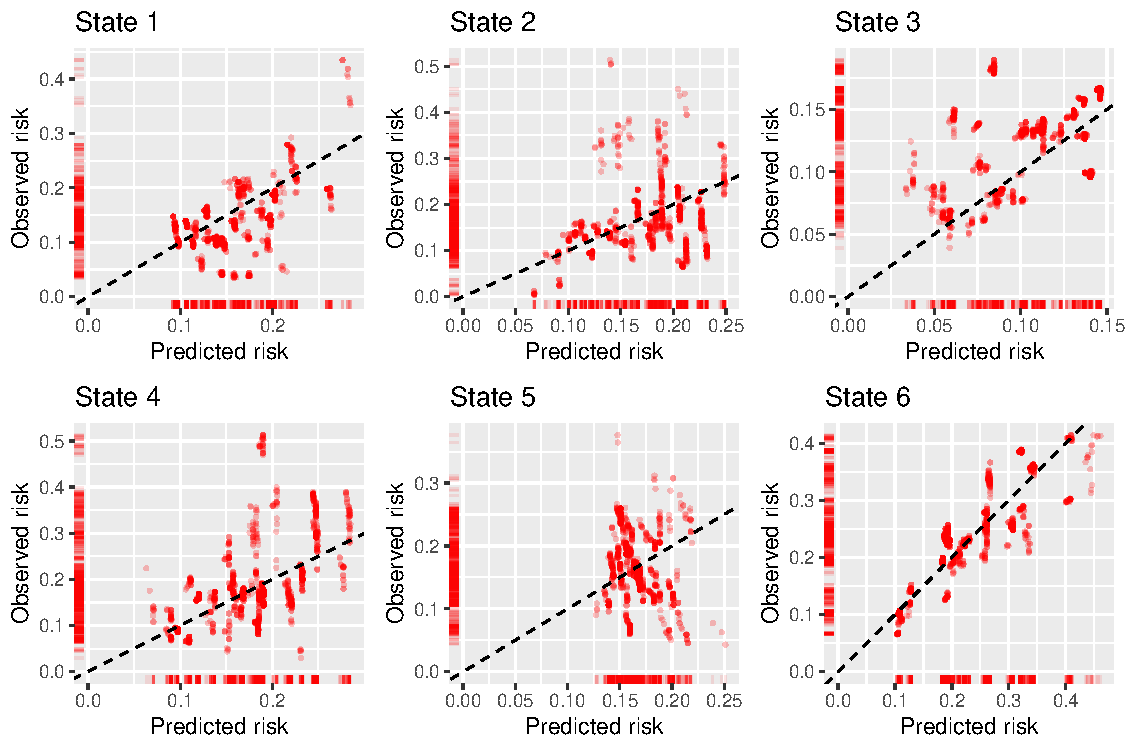
\includegraphics{calibmsm-jss-TEST-010}
\caption{\label{fig:mlrj1s0} MLR-IPCW calibration curves out of state j =  1 at time s = 0.}
\end{figure}

%% Subsection for s = 100
\subsection[Plots out of state j = 1 and 3 at time s = 100]{Plots out of state $j = 1$ and $3$ at time $s = 100$} \label{sec:plotss100}

In the work of \cite{DeWreede2011} focus then shifts to comparing transition probabilities when $s = 100$ depending on whether an individual has had an adverse event (state $3$) or remains in state $1$ (post transplant). Our focus therefore now shifts to assessing the calibration of these transition probabilities. This is done using the same approaches in combination with landmarking, as described in section \ref{sec:methodology}. In \pkg{calibmsm}, the process remains the same, changing the inputted values \code{j} and \code{s}, and providing the appropriate predicted transition probabilities into the argument \code{tp.pred}. We start by producing the calibration plots for $j = 1$ and $s = 100$ using the BLR-IPCW (Figure \ref{fig:blrj1s100}) and pseudo-value (Figure \ref{fig:pvj1s100}) methods. Given the small number of data points in this analysis induced by landmarking, we do not produce calibration scatter plots using MLR-IPCW.

\begin{Schunk}
\begin{Sinput}
R> dat.calib.blr.j1.s100 <-
+    calib_blr(data.mstate = msebmtcal,
+                   data.raw = ebmtcal,
+                   j=1,
+                   s=100,
+                   t.eval = t.eval,
+                   tp.pred = tps100 |>
+                     dplyr::filter(j == 1) |>
+                     dplyr::select(any_of(paste("pstate", 1:6, sep = ""))),
+                   curve.type = "rcs",
+                   rcs.nk = 3,
+                   w.covs = c("year", "agecl", "proph", "match"),
+                   CI = 95,
+                   CI.R.boot = 200)
R> dat.calib.pv.j1.s100 <-
+    calib_pv(data.mstate = msebmtcal,
+                  data.raw = ebmtcal,
+                  j=1,
+                  s=100,
+                  t.eval = t.eval,
+                  tp.pred = tps100 |>
+                   dplyr::filter(j == 1) |>
+                   dplyr::select(any_of(paste("pstate", 1:6, sep = ""))),
+                  curve.type = "rcs",
+                  rcs.nk = 3,
+                  group.vars = c("year"),
+                  CI = 95,
+                  CI.type = "parametric")
\end{Sinput}
\end{Schunk}

There are only four calibration plots because no individuals in state $j = 1$ at time $s = 100$ are in states $k = 3$ (adverse event) or $k = 4$ (recovery + adverse event) after $t = 1826$ days. The calibration of the predicted transition probabilities is very poor. Only for state $k = 6$ is the observed risk a monotonically increasing function of the predicted transition probability. We follow this up with the pseudo-value calibration plots (Figure \ref{fig:pvj1s100}) which leads to similar conclusions, as again only stat e$k = 6$ has a monotonically increasing calibration curve. The size of the confidence intervals are much larger than in the calibration plots for state $j = 1$ at time $s = 0$ (Figures \ref{fig:blrj1s0} and \ref{fig:pvj1s0}) for both the BLR-IPCW and pseudo-value approaches. For states $k = 2$ and $k = 5$, this could mean the poor calibration is a result of sampling variation as opposed to a misspecified model. A larger validation dataset would be required to get to the bottom of this. For state $k = 1$, the calibration is extremely poor and is unlikely driven by sampling variation.

\begin{figure}
\centering
\begin{Schunk}
\begin{Sinput}
R> plot(dat.calib.blr.j1.s100, combine = TRUE, nrow = 2, ncol = 2)
\end{Sinput}
\end{Schunk}
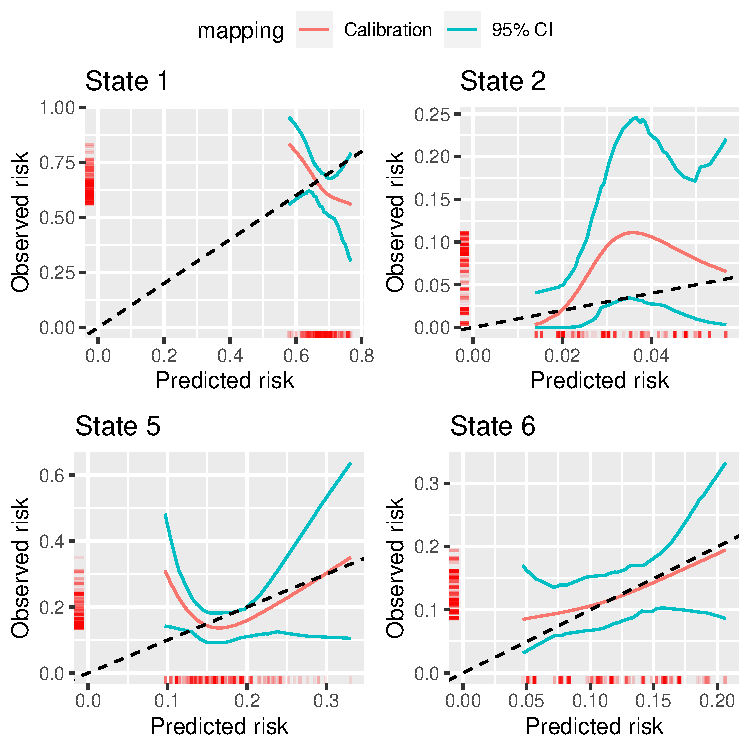
\includegraphics{calibmsm-jss-TEST-012}
\caption{\label{fig:blrj1s100} BLR-IPCW calibration curves out of state j =  1 at time s = 100.}
\end{figure}

\begin{figure}
\centering
\begin{Schunk}
\begin{Sinput}
R> plot(dat.calib.pv.j1.s100, combine = TRUE, nrow = 2, ncol = 2)
\end{Sinput}
\end{Schunk}
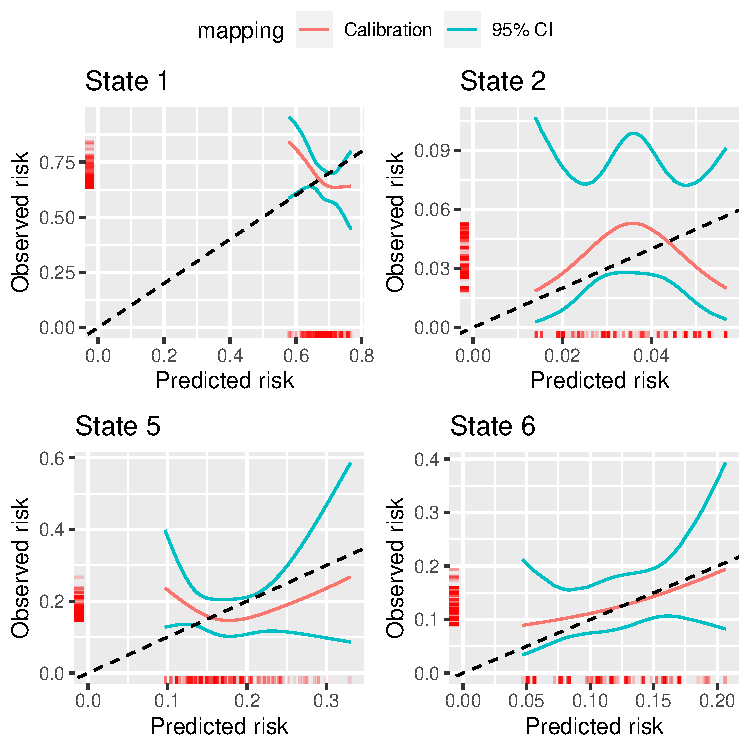
\includegraphics{calibmsm-jss-TEST-013}
\caption{\label{fig:pvj1s100} Pseudo-value calibration curves out of state j =  1 at time s = 100.}
\end{figure}

Next we produce calibration plots for $j = 3$ and $s = 100$ using the BLR-IPCW (Figure \ref{fig:blrj3s100}) and pseudo-value (Figure \ref{fig:pvj3s100}) methods.

\begin{Schunk}
\begin{Sinput}
R> dat.calib.blr.j3.s100 <-
+    calib_blr(data.mstate = msebmtcal,
+                   data.raw = ebmtcal,
+                   j=3,
+                   s=100,
+                   t.eval = t.eval,
+                   tp.pred = tps100 |>
+                     dplyr::filter(j == 3) |>
+                     dplyr::select(any_of(paste("pstate", 1:6, sep = ""))),
+                   curve.type = "rcs",
+                   rcs.nk = 3,
+                   w.covs = c("year", "agecl", "proph", "match"),
+                   CI = 95,
+                   CI.R.boot = 200)
R> dat.calib.pv.j3.s100 <-
+    calib_pv(data.mstate = msebmtcal,
+                  data.raw = ebmtcal,
+                  j=3,
+                  s=100,
+                  t.eval = t.eval,
+                  tp.pred = tps100 |>
+                   dplyr::filter(j == 3) |>
+                   dplyr::select(any_of(paste("pstate", 1:6, sep = ""))),
+                  curve.type = "rcs",
+                  rcs.nk = 3,
+                  group.vars = c("year"),
+                  CI = 95,
+                  CI.type = "parametric")
\end{Sinput}
\end{Schunk}

Again there are only four possible states that an individual may transition into, although this includes states $3$ (adverse event) and $4$ (recovery + adverse event), instead of $1$ (post transplant) and $2$ (recovery). The calibration plots are better than for $j = 1$. For transitions into states $k = 3, 4$ and $6$, the calibration curves are monotonically increasing and the confidence interval contains the entire line of perfect calibration. This is true when calibration is assessed using BLR-IPCW or pseudo-values. Again the calibration of state $5$ is very poor. This makes it difficult to base any clinical decisions on the predicted transition probabilities for relapse out of states $j = 1$ or $3$ at time $s = 100$, whereas making clinical decisions based on the risk of death ($k = 6$) after survival for $100$ days is more viable, as this was well calibrated for both $j = 1$ and $j = 3$. With the exception of the transition probabilities from $j = 1$ into state $k = 3$ made at time $s = 0$, there has been broad agreement between the calibration curves estimated using the BLR-IPCW and pseudo-value approaches. This provides some evidence about the assessment of calibration, and that the assumptions on which each method is based are satisfied.

\begin{figure}
\centering
\begin{Schunk}
\begin{Sinput}
R> plot(dat.calib.blr.j3.s100, combine = TRUE, nrow = 2, ncol = 2)
\end{Sinput}
\end{Schunk}
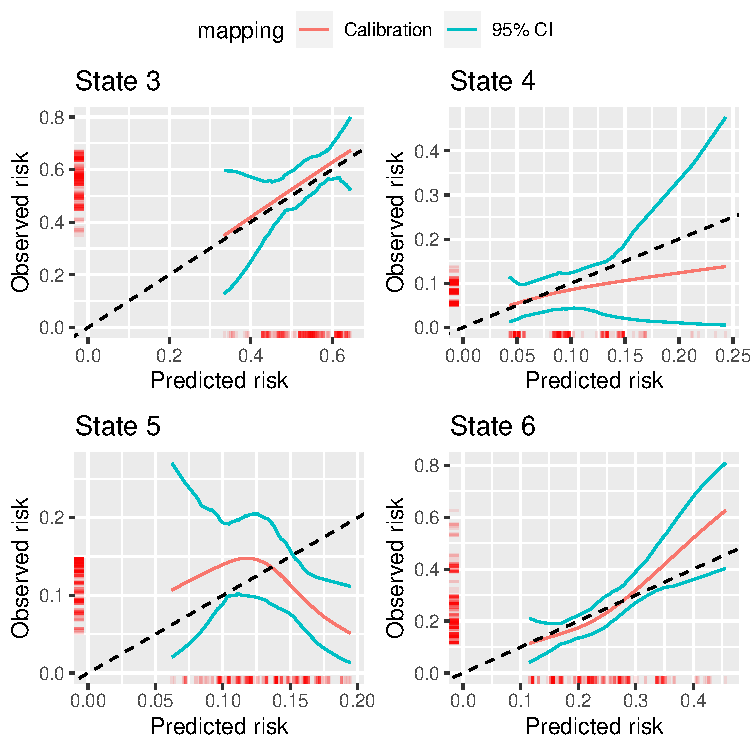
\includegraphics{calibmsm-jss-TEST-015}
\caption{\label{fig:blrj3s100} BLR-IPCW calibration curves out of state j =  3 at time s = 100.}
\end{figure}

\begin{figure}
\centering
\begin{Schunk}
\begin{Sinput}
R> plot(dat.calib.pv.j3.s100, combine = TRUE, nrow = 2, ncol = 2)
\end{Sinput}
\end{Schunk}
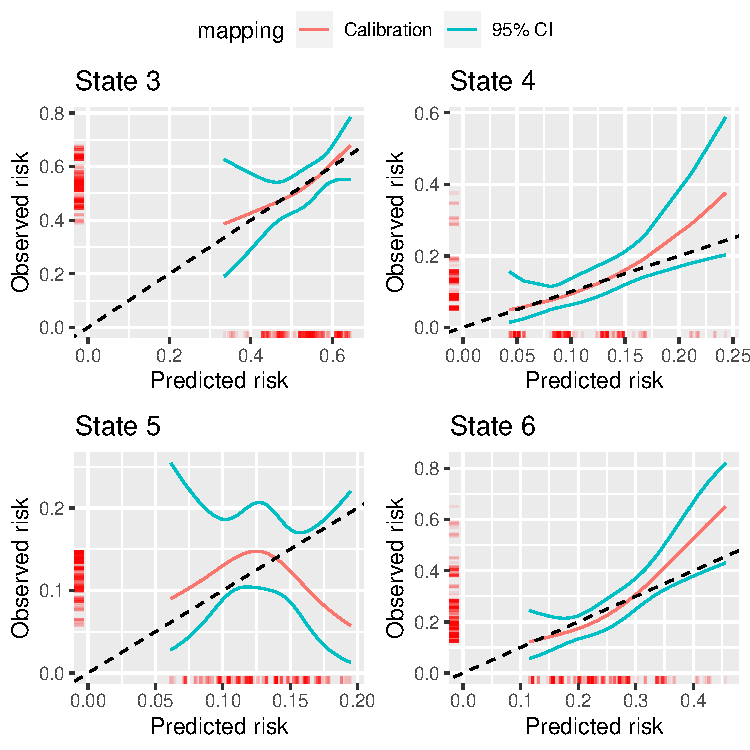
\includegraphics{calibmsm-jss-TEST-016}
\caption{\label{fig:pvj3s100} Pseudo-value calibration curves out of state j =  3 at time s = 100.}
\end{figure}

%% Section 5 - Discussion
%
% \section{Discussion} \label{sec:discussion}
%
% Multistate models are a unique tool for prediction, allowing risks to be updated after key events happen post baseline. Development of multistate models for prediction is becoming more common, yet validation of such models is still very uncommon. A major barrier to implementation of statistical techniques is often the availability of software \citep{Pullenayegum2016}. \pkg{calibmsm} has been developed to aid in the implementation of techniques to assess the calibration of transition probabilities from a multistate model. This paper has extended previously proposed methods for assessing the calibration of the transition probabilities out of the initial state \textbf{XXXX REF PROJECT 6}, to the transition probabilities out of any state $j$ at any time $s$.
%
% All three methods (BLR-IPCW, MLR-IPCW and pseudo-value) have been shown to give an unbiased assessment of calibration under non-informative censoring mechanisms, and a predominately unbiased assessment of calibration under strongly informative censoring \textbf{XXXX REF PROJECT 6}. This paper found broadly similar evaluation of calibration when using the BLR-IPCW and pseudo-value methods, however there were discrepancies in the evaluation of calibration of the transition probabilities into state $k = 3$. Further research evaluating these methods performance in a wider range of simulation scenarios, and by a different research group \citep{Boulesteix2013}, would be highly valuable \citep{Heinze2022}.
%
% It is also possible to use the \pkg{calibmsm} to validate competing risks models, which are a special case of a multistate models. However, graphical calibration curves already exist for assessing the calibration of a competing risks model \citep{Austin2022}. When fitting graphical calibration curves, it is assumed that censoring is independent of the outcome after conditioning on the complementary log-log transformation of the predicted risk, and the assumption of proportional hazards is made. When implementing BLR-IPCW, the assumption of independence between the censoring mechanism and the outcome in the reweighted population is made. For the pseudo-value approach, censoring is assumed to be non-informative within the specified subgroups. These are different approaches to dealing with the issue of informative censoring in the validation dataset when assessing the calibration of the model. We carried out a sensitivity analyses, comarping BLR-IPCW, pseudo-values and graphical calibration curves for assessing the calibration of a competing risks model out of the first state (post transplant) using the EBMT data \citep{EBMT2023}. This is contained in a vignette \emph{'comparison with graphical calibration curves'} provided with the package. All methods resulted in similar calibration curves, but the relative performance of each methods in a wider range of scenarios is still unknown. A comparison of these methods in a simulation when the aforementioned assumptions do and do not hold, and under a range of sample sizes and multistate model structures, would be therefore valuable. Both of these recommendations for future work would constitute phase 3 and 4 studies in the evidence base for new methods \citep{Heinze2022}.
%
% The BLR-IPCW and pseudo-value approaches have different computational burdens. A calibration curve can be obtained reasonably quickly using the BLR-IPCW approach, however because bootstrapping is the preferred method for estimating the confidence interval \ref{sec:ci}, which will result in a high computational burden in large validation datasets. On the contrary, obtaining the calibration curve using the pseudo-value approach has a high computational burden due to calculation of the pseudo-values themselves. Once these have been calculated, a calibration curve and confidence interval can be estimated quickly using parametric techniques, meaning estimation of the confidence interval adds minimal computational burden. We plan to extend the package to allow users to estimate the pseudo-values for each individual seperately before estimating the calibration curve. This will allow the first part of the process to be parallelised and makes estimation of calibration curves using the pseudo-value approach more feasible in large datasets.
%
% Estimation of the weights is clearly of high importance for the BLR-IPCW and MLR-IPCW approaches. If the model to do so is misspecified, this could lead to incorrect evaluation of the calibration. It is possible this is what is causing the difference between BLR-IPCW and pseudo-value for the calibration of transition probabilities from staet $j = 1$ at time $s = 0$ into state $k = 3$. This package is focused on creation of calibration curves, but is not a dedicated package for estimating inverse probability of censoring weights. We encourage the user to create a well specified model for the weights. Custom functions for estimating the weights can be specified through the \code{w.function} argument in both \code{calib_blr} and \code{calib_mlr}. Alternatively, weights can be estimated externally and then specified though the \code{weights} argument. In this latter case, the internal bootstrapping procedure will not work, as the weights need to be re-estimated in each bootstrap dataset. We have provided a more detailed vignette about how to estimate calibration curves and confidence intervals using bootstrapping when defining your own function to estimate the weights (\emph{BLR-IPCW-manual-bootstrap-with-custom-function-for-estimating-the-weights}).
%
% In summary, \pkg{calibmsm} provides tools to assess the calibration of the transition probabilities of a multistate model or competing risks model using three approaches (BLR-IPCW, MLR-IPCW and pseudo-values). Further comparison of these approaches in targeted simulations to establish their performance under different censoring mechanisms and assumptions would be valuable.
%
% %% -- Optional special unnumbered sections -------------------------------------
%
% \section*{Computational details}
%
% \textbf{WILL UPDATE THIS SECTION ONCE PACKAGE HAS BEEN FINALISED AND UPLOADED TO CRAN}
%
% The results in this paper were obtained using
% \proglang{R}~4.3.0 with the
% \pkg{dplyr}~1.1.2,
% \pkg{tidyr}~1.3.0,
% \pkg{ggplot2}~3.4.2,
% \pkg{ggpubr}~0.6.0,
% \pkg{Hmisc}~5.0.1,
% \pkg{rms}~6.6.0,
% \pkg{VGAM}~1.1.8,
% \pkg{boot}~1.3.28.1,
% \pkg{survival}~3.5.5,
% \pkg{stats}~4.3.0,
% \pkg{magrittr}~2.0.3. \proglang{R} itself
% and all packages used are available from the Comprehensive
% \proglang{R} Archive Network (CRAN) at
% \url{https://CRAN.R-project.org/}.
%
% \section*{Acknowledgments}
%
% \begin{leftbar}
% Thank you to Thomas Yee for helping to debug an issue with implementing vector spline smoothers from the \pkg{VGAM} package within \pkg{calibmsm}.
% \end{leftbar}
%
\bibliography{refs}

%% -- Appendix (if any) --------------------------------------------------------
%% - After the bibliography with page break.
%% - With proper section titles and _not_ just "Appendix".

% \newpage
%
% \begin{appendix}
%
% \begin{leftbar}
% Appendices can be included after the bibliography (with a page break). Each
% section within the appendix should have a proper section title (rather than
% just \emph{Appendix}).
%
% For more technical style details, please check out JSS's style FAQ at
% \url{https://www.jstatsoft.org/pages/view/style#frequently-asked-questions}
% which includes the following topics:
% \begin{itemize}
%   \item Title vs.\ sentence case.
%   \item Graphics formatting.
%   \item Naming conventions.
%   \item Turning JSS manuscripts into \proglang{R} package vignettes.
%   \item Trouble shooting.
%   \item Many other potentially helpful details\dots
% \end{itemize}
% \end{leftbar}
%
%
% \section[Using BibTeX]{Using \textsc{Bib}{\TeX}} \label{app:bibtex}
%
% \begin{leftbar}
% References need to be provided in a \textsc{Bib}{\TeX} file (\code{.bib}). All
% references should be made with \verb|\cite|, \verb|\citet|, \verb|\citep|,
% \verb|\citealp| etc.\ (and never hard-coded). This commands yield different
% formats of author-year citations and allow to include additional details (e.g.,
% pages, chapters, \dots) in brackets. In case you are not familiar with these
% commands see the JSS style FAQ for details.
%
% Cleaning up \textsc{Bib}{\TeX} files is a somewhat tedious task -- especially
% when acquiring the entries automatically from mixed online sources. However,
% it is important that informations are complete and presented in a consistent
% style to avoid confusions. JSS requires the following format.
% \begin{itemize}
%   \item JSS-specific markup (\verb|\proglang|, \verb|\pkg|, \verb|\code|) should
%     be used in the references.
%   \item Titles should be in title case.
%   \item Journal titles should not be abbreviated and in title case.
%   \item DOIs should be included where available.
%   \item Software should be properly cited as well. For \proglang{R} packages
%     \code{citation("pkgname")} typically provides a good starting point.
% \end{itemize}
% \end{leftbar}
%
% \end{appendix}

%% -----------------------------------------------------------------------------


\end{document}
